%
% spektral.tex -- spektrale Graphentheorie
%
% (c) 2020 Prof Dr Andreas Müller, Hochschule Rapperswil
%
\section{Spektrale Graphentheorie
\label{buch:section:spektrale-graphentheorie}}
\rhead{Spektrale Graphentheorie}
Die Adjazenzmatrix, die Gradmatrix und damit natürlich auch
die Laplace-Matrix codieren alle wesentliche Information eines
ungerichteten Graphen.
Sie operiert auf Vektoren, die für jeden Knoten des Graphen eine
Komponente haben.
Dies eröffnet die Möglichkeit, den Graphen über die linearalgebraischen
Eigenschaften dieser Matrizen zu studieren.
Dieser Abschnitt soll diese Idee an dem ziemlich übersichtlichen Beispiel
der chromatischen Zahl eines Graphen illustrieren.

\subsection{Chromatische Zahl und Unabhängigkeitszahl
\label{buch:subsection:chromatische-zahl}}
Der Grad eines Knotens ist ein Mass dafür, wie stark ein Graph
``vernetzt'' ist.
Je höher der Grad, desto mehr direkte Verbindungen zwischen Knoten gibt es.
Noch etwas präziser kann diese Idee die mit Hilfe der 
chromatischen Zahl und der Unabhängigkeitszahl erfasst werden.

\begin{definition}
Die {\em chromatische Zahl} $\operatorname{chr}G$ eines Graphen $G$ ist
die minimale Anzahl von Farben, die zum Einfärben der Knoten eines Graphen
nötig sind, sodass benachbarte Knoten verschiedene Farben haben.
\index{chromatische Zahl}
\end{definition}

\begin{definition}
Eine Menge von Knoten eines Graphen heisst {\em unabhängig}, wenn 
keine zwei Knoten der Menge im Graphen verbunden sind.
Die {\em Unabhängigkeitszahl} $\operatorname{ind}G$ eines Graphen $G$
ist die maximale Anzahl Knoten einer unabhängigen Menge.
\index{Unabhängigkeitszahl}
\end{definition}

\begin{beispiel}
Abbildung~\ref{buch:graphen:fig:chrindpeterson} bestimmt die chromatische
Zahl und die Unabhängigkeitszahl im Beispiel des Peterson-Graphen.
\end{beispiel}

Zwischen der chromatischen Zahl und der Unabhängigkeitszahl eines Graphen
muss es einen Zusammenhang geben.
Je mehr Verbindungen es im Graphen gibt, desto grösser wird die chromatische
Zahl.
Gleichzeitig wird es schwieriger für Mengen von Knoten, unabhängig zu sein.

\begin{satz}
\label{buch:satz:chrind}
Ist $G$ ein Graph mit $n$ Knoten, dann gilt
$\operatorname{chr}G\cdot\operatorname{ind}G\ge n$.
\end{satz}

\begin{proof}[Beweis]
Eine minimale Färbung des Graphen mit $\operatorname{chr}G$ Farben
teilt die Knoten in $\operatorname{chr}G$ disjunkte Mengen $V_f$ von Knoten mit
gleicher Farbe $f$ ein.
Da diese Mengen einfarbig sind, sind sie unabhängig, enthalten also
höchstens so viele Knoten, wie die Unabhängigkeitszahl erlaubt,
also $|V_f|\le \operatorname{ind}G$.
Da die Menge aller Knoten die Vereinigung der Mengen $V_f$ ist,
ist die Gesamtzahl der Knoten 
\begin{align*}
V
&=
\bigcup_{\text{$f$ eine Farbe}} V_f
&&\Rightarrow&
n
&=
\sum_{\text{$f$ eine Farbe}} |V_f| 
\\
&
&&&
&\le
\sum_{\text{$f$ eine Farbe}} \operatorname{ind}G
=
(\text{Anzahl Farben})\cdot \operatorname{ind}G
=
\operatorname{chr}G \cdot \operatorname{ind}G.
\end{align*}
Damit ist $n\le \operatorname{chr}G\cdot\operatorname{ind}G$ gezeigt.
\qedhere
\end{proof}

\begin{beispiel}
In einem vollständigen Graphen ist jeder Knoten mit jedem anderen verbunden.
Jede Menge mit zwei oder mehr Knoten kann daher nicht unabhängig sein, die
Unabhängigkeitszahl ist daher $\operatorname{ind}G=1$.
Andererseits ist für jeden Knoten eine eigene Farbe nötig, daher ist die
chromatische Zahl $\operatorname{chr}G=n$.
Die Ungleichung von Satz~\ref{buch:satz:chrind} ist erfüllt, sogar mit
Gleichheit.
Das Beispiel zeigt, dass die Ungleichung nicht ohne zusätzliche Annahmen
verbessert werden kann.
\end{beispiel}

\begin{figure}
\centering
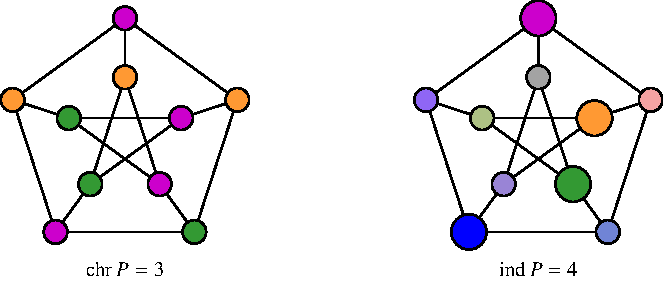
\includegraphics{chapters/70-graphen/images/petersonchrind.pdf}
\caption{Chromatische Zahl und Unabhängigkeitszahl des Peterson-Graphen.
Die chromatische Zahl ist $3$, da der Graph sich mit drei Farben einfärben
lässt (links).
Die Unabhängigkeitszahl ist $4$, die vier grösseren Knoten im rechten
Graphen sind unabhängig.
Die Farben der kleinen Knoten sind die additive Mischung der Farben
der grossen Knoten, mit denen sie verbunden sind.
\label{buch:graphen:fig:chrindpeterson}}
\end{figure}

\begin{beispiel}
Der Peterson-Graph $P$ von Abbildung~\ref{buch:graphen:fig:chrindpeterson}
hat chromatische Zahl $\operatorname{chr}P=3$ und Unabhängigkeitszahl
$\operatorname{ind}P=4$.
Die Ungleichung von Satz~\ref{buch:satz:chrind} ist erfüllt, sogar als
Ungleichung: $\operatorname{chr}P\cdot\operatorname{ind}P=3\cdot 4=12>10=n$.
\end{beispiel}

Nach Definition ist die Unabhängigkeitszahl ein Mass für die Grösse einer
unabhängigen Menge von Punkten.
Der Beweis von Satz~\ref{buch:satz:chrind} zeigt, dass man sich die
chromatische Zahl als ein Mass dafür vorstellen kann,
wieviele solche unabhängige 
Mengen in einem Graphen untergebracht werden können.

%
% Chromatische Zahl und maximaler Grad
%
\subsection{Chromatische Zahl und maximaler Grad
\label{buch:subsection:chr-und-maximaler-grad}}
Wenn kein Knoten mehr als $d$ Nachbarn hat, dann reichen
$d+1$ Farben immer, um diesen Knoten und seine Nachbarn einzufärben.
Das heisst aber noch nicht, dass dann auch $d+1$ Farben zur
Einfärbung des ganzen Graphen reichen.
Genau dies garantiert jedoch der folgende Satz.

\begin{definition}
Der {\em maximale Grad}
\(
\max_{v\in V} \deg(v)
\)
eines ungerichteten Graphen 
wird mit $d$ bezeichnet.
\index{maximaler Grad}%
\end{definition}

\begin{satz}
\label{buch:graphen:satz:chrmaxgrad}
Ist $G$ ein Graph mit maximalem Grad $d$, dann gilt 
$\operatorname{chr}G \le d+1$.
\end{satz}

\begin{proof}[Beweis]
Wir führen den Beweis mit Hilfe von vollständiger Induktion nach der
Anzahl Knoten eines Graphen.
Ein Graph mit nur einem Knoten hat keine Kanten, der maximale Grad ist
daher $d=0$ und $d+1=1$ Farbe reicht auch tatsächlich zur Einfärbung des
einen Knotens.

Wir nehmen jetzt an, die Behauptung sei für Graphen mit $n-1$ Knoten bereits
bewiesen, ein Graph $G'$ mit $n-1$ Knoten und maximalem Grad $d'$ erfüllt
also die Ungleichung $\operatorname{chr}G'\le d'+1$.

Wir wählen jetzt einen beliebigen Knoten $v$ des Graphen $G$ und bilden
den Graphen $G'$, der aus $G$ entsteht, indem man den Knoten $v$
entfernt: $G'=G\setminus\{v\}$.
Der maximale Grad $d'$ von $G'$ kann dabei nicht grösser werden, es ist
also $d'\le d$.
Da $G'$ genau $n-1$ Knoten hat, lässt er sich mit höchstens $d'+1\le d+1$
Farben einfärben.
Es muss jetzt also nur noch eine Farbe für den Knoten $v$ gefunden werden.
Da $d$ der maximale Grad ist, hat $v$ höchstens $d$ Nachbarn, die höchstens
$d$ verschiedene Farben haben können.
Von den $d+1$ zur Verfügung stehenden Farben bleibt also mindestens eine
übrig, mit der man den Knoten $v$ einfärben kann.
Damit ist der Induktionsschritt gelungen und somit der Satz bewiesen.
\end{proof}

Das Argument im Beweis von Satz~\ref{buch:graphen:satz:chrmaxgrad}
ist für alle Begriffe anwendbar, die sich bei der Bildung eines 
Untergraphen auf ``monotone'' Art ändern.
Die chromatische Zahl eines Untergraphen ist höchstens so gross wie die
des ganzen Graphen. 
Daher kann man eine Ungleichung für grosse Graphen schrittweise aus
entsprechenden Ungleichungen für die kleineren Teilgraphen gewinnen.
Ziel der folgenden Abschnitte ist zu zeigen, dass sich eine Grösse
mit ähnlichen Eigenschaften aus dem Eigenwertspektrum der Adjazenzmatrix
ablesen lässt.
Daraus ergibt sich dann eine bessere Abschätzung der chromatischen Zahl
eines Graphen.

%
% maximaler Eigenwert und maximaler Grad
%
\subsection{Maximaler Eigenwert von $A(G)$ und maximaler Grad
\label{buch:subsection:maximaler-eigenwert}}
Die Adjazenzmatrix $A(G)$ eines Graphen $G$  mit $n$ Knoten enthält unter
anderem auch die Information über den Grad eines Knotens.
Die Summe der Elemente einer Zeile oder einer Spalte ergibt einen Vektor,
der die Grade der Knoten als Komponenten enthält.
Ist $U$ ein $n$-dimensionaler Vektor aus lauter Einsen, dann ist
ist $A(G)U$ ein Spaltenvektor bestehend aus den Zeilensummen der Matrix 
$A(G)$ und
$U^tA(G)$ ein Zeilenvektor bestehend aus den Spaltensummen.
$A(G)U$ ist also der Vektor der Grade der Knoten.

Das Skalarprodukt von $A(G)U$ mit $U$ ist die Summe der Grade.
Somit ist
\begin{equation}
\frac{\langle A(G)U,U\rangle}{\langle U,U\rangle}
=
\frac{1}{\langle U,U\rangle}\sum_{v\in V}\deg(v)
=
\frac{1}{n}(d_1+\dots+d_n)
\label{buch:graphen:eqn:AUdavg}
\end{equation}
der {\em mittlere Grad}, der mit $\overline{d}$ bezeichnet werden soll.
Da die Kanten eines Graphen zusammen $2\cdot|E|$ Enden haben, kann
er auch als
\[
\overline{d}=\frac{2\cdot|E|}{|V|}
\]
berechnet werden.
\index{mittlerer Grad}%

Da $A(G)$ eine symmetrische Matrix ist, ist $A(G)$ diagonalisierbar,
die Eigenwerte sind also alle reell.
Es ist ausserdem bekannt, dass der Eigenvektor $f$ zum grössten Eigenwert
$\alpha_{\text{max}}$ von $A(G)$
den Bruch
\[
\frac{\langle A(G)f,f\rangle}{\langle f,f\rangle}
\]
für Vektoren $f\ne 0$ maximiert.
Aus~\eqref{buch:graphen:eqn:AUdavg} folgt damit, dass
\begin{equation}
\overline{d}
\le
\alpha_{\text{max}}
\label{buch:graphen:eqn:dqueramax}
\end{equation}
ist.

In Abschnitt~\ref{buch:section:positive-vektoren-und-matrizen}
des nächsten Kapitels wird die Perron-Frobenius-Theorie positiver
\index{Perron-Frobenius-Theorie}%
\index{positive Matrix}%
Matrizen vorgestellt, welche einer Reihe interessanter Aussagen
über den betragsgrössten Eigenwert und den zugehörigen Eigenvektor
macht.
Die Adjazenzmatrix ist eine nichtnegative Matrix und $\alpha_{\text{max}}$
ist der grösste Eigenwert, also genau die Grösse, auf die die
Sätze~\ref{buch:wahrscheinlichkeit:satz:perron-frobenius}
und \ref{buch:wahrscheinlichkeit:satz:perron-frobenius2}
anwendbar sind.
Dazu muss die Matrix allerdings primitiv sein
(Definition~\ref{buch:positiv:def:primitiv} in Kapitel~\ref{buch:chapter:wahrscheinlichkeit}),
was gleichbedeutend
\index{primitive Matrix}%
ist damit, dass der Graph zusammenhängend ist.
Im folgenden soll dies daher jeweils angenommen werden.

\begin{satz}
Ist $G$ ein zusammenhängender Graph mit $n$ Knoten und maximalem Grad $d$,
dann gilt
\[
\frac1n\sum_{v\in V} \deg(v) 
=
\overline{d}
\le \alpha_{\text{max}} \le d.
\]
\end{satz}

\begin{proof}[Beweis]
Wir wissen aus \eqref{buch:graphen:eqn:dqueramax} bereits, dass
$\overline{d}\le\alpha_{\text{max}}$ gilt, es bleibt also nur noch
$\alpha_{\text{max}}\le d$ zu beweisen.

Sei $f$ der Eigenvektor zum Eigenwert $\alpha_{\text{max}}$.
Nach Satz~\label{buch:wahrscheinlichkeit:satz:perron-frobenius2}
ist $f$ ein positiver Vektor mit der Eigenschaft $A(G)f=\alpha_{\text{max}}f$.
Der Eigenvektor $f$ ist eine Funktion auf den Knoten des Graphen,
die $v$-Komponente des Vektors $f$ für einen Vertex $v\in V$ ist $f(v)$.
Die Eigenvektoreigenschaft bedeutet $(A(G)f)(v)=\alpha_{\text{max}} f(v)$.
Die Adjazenzmatrix $A(G)$ enthält in Zeile $v$ genau für diejenigen
Knoten $u\in V$ Einsen, die zu $v$ benachbart sind.
Schreiben wir $u\sim v$ für die Nachbarschaftsrelation, dann ist 
\[
(A(G)f)(v)
=
\sum_{u\sim v} f(u).
\]
Die Summe der Komponenten $A(G)f$ kann man durch Multiplikation
von $A(G)f$ mit einem Zeilenvektor $U^t$ aus lauter Einsen erhalten, also
\begin{equation}
\begin{aligned}
{\color{red}
\sum_{v\in V}}\sum_{u\sim v}f(v)
&=
{\color{red}U^t}A(G)f
=
(U^tA(G))f
=
\begin{pmatrix}d_1&d_2&\dots&d_n\end{pmatrix} f
\\
&=
\sum_{v\in V}\deg (v) f(v)
\le
\sum_{v\in V}df(v)
=
d
\sum_{v\in V}f(v).
\end{aligned}
\label{buch:graphen:eqn:sumkomp}
\end{equation}
Andererseits ist $A(G)f=\alpha_{\text{max}}f$, die linke Seite
von~\eqref{buch:graphen:eqn:sumkomp} ist daher
\begin{equation}
\sum_{v\in V}\sum_{u\sim v}f(v)
=
U^tA(G)f
=
\alpha_{\text{max}}
U^tf
=
\alpha_{\text{max}} \sum_{v\in V}f(v).
\label{buch:graphen:eqn:sumkomp2}
\end{equation}
Die Ungleichung~\eqref{buch:graphen:eqn:sumkomp}
und die Gleichung~\eqref{buch:graphen:eqn:sumkomp2} ergeben zusammen
die Ungleichung
\[
\alpha_{\text{max}} \sum_{v\in V}f(v)
\le d\sum_{v\in V}f(v)
\qquad\Rightarrow\qquad
\alpha_{\text{max}} \le d,
\]
da die Summe der Komponenten des positiven Vektors $f$ nicht verschwinden
kann.
Damit ist die Ungleichung bewiesen.
\end{proof}

%
% alpha_max eines Untergraphen
%
\subsection{$\alpha_{\text{max}}$ eines Untergraphen
\label{buch:subsection:alphamax-eines-untergraphen}}
Der grösste Eigenwert $\alpha_{\text{max}}$ ist ein potentieller 
Anwärter für eine bessere Abschätzung der chromatischen Zahl.
Bereits früher wurde bemerkt, dass dies auch bedeutet, dass man 
das Verhalten des grössten Eigenwerts bei einem Übergang zu einem
Untergraphen verstehen muss.

\begin{satz}
\label{buch:graphen:satz:amaxuntergraph}
Sei $G'$ ein echter Untergraph von $G$ mit Adjazenzmatrix $A(G')$ und
grösstem Eigenwert $\alpha_{\text{max}}'=\varrho(A(G'))$, dann ist
$\alpha_{\text{max}}' \le \alpha_{\text{max}}$.
\end{satz}

\begin{proof}[Beweis]
Sei $f'$ der positive Eigenvektor zum Eigenwert $\alpha_{\text{max}}'$
der Matrix $A(G')$.
$f'$ ist definiert auf der Menge $V'$ der Knoten von $G'$.
Aus $f'$ lässt sich ein Vektor $g$ mit den Werten
\[
g(v)
=
\begin{cases}
f'(v)&\qquad v\in V'\\
    0&\qquad\text{sonst}
\end{cases}
\]
konstruieren, der auf ganz $V$ definiert ist.

Die Vektoren $f'$ und $g$ haben auf $V'$ die gleichen Komponenten, also ist auch
$\langle f',f'\rangle = \langle g,g\rangle$.
Die Matrixelemente von $A(G')$ und $A(G)$ auf gemeinsamen Knoten $u,v\in V'$ 
erfüllen $A(G')_{uv}\le A(G)_{uv}$, da jede Kante von $G'$ auch in $G$ ist.
Daher gilt
\[
\langle A(G')f',f'\rangle
\le
\langle A(G)g,g\rangle,
\]
woraus sich die Ungleichung
\[
\alpha_{\text{max}}'
=
\frac{\langle A(G')f',f'\rangle}{\langle f',f'\rangle}
=
\frac{\langle A(G)g,g\rangle}{\langle g,g\rangle}
\le
\alpha_{\text{max}}
\]
ergibt, da $\alpha_{\text{max}}$ das Maximum von
$\langle A(G)h,h\rangle/\langle h,h\rangle$ für alle Vektoren $h\ne 0$ ist.
\end{proof}

%
% Der Satz von Wilf
%
\subsection{Chromatische Zahl und $\alpha_{\text{max}}$: Der Satz von Wilf
\label{buch:subsection:chr-und-alpha-max}}
\index{Satz von Wilf}%
\index{Wilf, Satz von}%
Die in Satz~\ref{buch:graphen:satz:amaxuntergraph} beschriebene
Eigenschaft von $\alpha_{\text{max}}$ beim Übergang zu einem Untergraphen
ermöglich jetzt, eine besser Abschätzung für die chromatische Zahl
zu finden.

\begin{satz}[Wilf]
\label{buch:graphen:satz:wilf}
Sie $G$ ein zusammenhängder Graph und $\alpha_{\text{max}}$ der grösste
Eigenwert seiner Adjazenzmatrix. Dann gilt
\[
\operatorname{chr}G\le \alpha_{\text{max}}+1.
\]
\end{satz}

\begin{proof}[Beweis]
Wie der Satz~\ref{buch:graphen:satz:chrmaxgrad} kann auch der Satz von Wilf
mit Hilfe von vollständiger Induktion über die Anzahl $n$ der Knoten
bewiesen werden.

Ein Graph mit nur einem Knoten hat die $0$-Matrix als Adjazenzmatrix,
der maximale Eigenwert ist $\alpha_{\text{max}}=0$, und tatsächlich reicht
$\alpha_{\text{max}}+1=1$ Farbe, um den einen Knoten einzufärben.
Dies ist die Induktionsverankerung.

Im Sinne der Induktionsannahme 
nehmen wir jetzt an, der Satz sei für Graphen mit $n-1$ Knoten bereits
beweisen.
Wir müssen dann zeigen, dass der Satz dann auch für Graphen mit $n$ Knoten
gilt.

Sei $v\in V$ ein Knoten minimalen Grades und $G'=G\setminus\{v\}$ der
Untergraph, der entsteht, wenn der Knoten $v$ entfernt wird.
Da $G'$ genau $n-1$ Knoten hat, gilt der Satz von Wilf für $G'$
und daher kann $G'$ mit höchstens
\[
\operatorname{chr}G' \le 1 + \alpha_{\text{max}}'
\]
Farben eingefärbt werden.
Nach Satz~\ref{buch:graphen:satz:amaxuntergraph} ist
$\alpha_{\text{max}}'\le \alpha_{\text{max}}$,
Also kann $G'$ mit höchstens $\alpha_{\text{max}}+1$ Farben eingefärbt werden.

Da $v$ ein Knoten minimalen Grades ist, ist sein Grad
$d(v)\le \overline{d}\le \alpha_{\text{max}}$.
Die Nachbarn von $v$ haben also hächstens $\alpha_{\text{max}}$ verschiedene
Farben, mit einer weiteren Farbe lässt sich also auch $G$ einfärben.
Daraus folgt $\operatorname{chr}G\le \alpha_{\text{max}}+1$.
\end{proof}

\begin{figure}
\centering
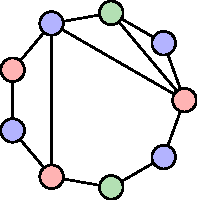
\includegraphics{chapters/70-graphen/images/nine.pdf}
\caption{Beispiel für einen Graphen, für den der
Satz~\ref{buch:graphen:satz:wilf} von Wilf die bessere
Abschätzung für die chromatische Zahl eines Graphen gibt als der
maximale Grad.
\label{buch:graphen:fig:wilfexample}}
\end{figure}

\begin{beispiel}
Der Graph in Abbildung~\ref{buch:graphen:fig:wilfexample} hat 12 Kanten und 9
Knoten, daher ist $\overline{d}\le \frac{24}{9}$.
Der maximale Grad ist $4$ und durch explizite Rechnung mit Hilfe zum Beispiel
von Octave ergibt, dass $\alpha_{\text{max}}\approx 2.9565$.
Aus dem Satz von Wilf folgt, dass
$\operatorname{chr}G\le \alpha_{\text{max}}+1$, und daraus ergibt sich
$\operatorname{chr}G\le 3$.
Tatsächlich ist die chromatische Zahl $\operatorname{chr}G=3$, da 
der Graph mindestens ein Dreieck enthält.
Der maximale Grad ist 4, somit gibt der
Satz~\ref{buch:graphen:satz:chrmaxgrad}
die Schranke 
$\operatorname{chr}G\le 4+1=5$
für die chromatische Zahl.
Der Satz von Wilf ist also eine wesentliche Verbesserung, er liefert in
diesem Fall den exakten Wert der chromatischen Zahl.
\end{beispiel}



